\documentclass[lecture,12pt,]{pcms-l}
\input preamble.tex
\input header.tex

%%%%%%%%%%%%%%%%%%%%%%%%%%%%%%%%%%%%%%%%%%%%%%%%%%%%%%%%%%%%%

\begin{document}
\mainmatter
\setcounter{page}{1}

\lectureseries[\course]{\course}

\auth[\lecAuth]{Lecturer: \lecAuth\\ Scribe: \scribe}
\date{October 27, 2009}

\setaddress

% the following hack starts the lecture numbering at 9
\setcounter{lecture}{8}
\setcounter{chapter}{8}

\lecture{Dynamics of Markov Chains}

\section{Discrete Space, Discrete Time Markov Chains}
Continuous time Markov chains exist but we will only be considering discrete time in this course. A Markov chain, $\mathbb{X}$, in discrete time could be $\mathbb{X}\in\mathbb{N}=\{1,2,3,\ldots\}$. Mostly we will restrict our discussion to a finite state space such that $\mathbb{X}=\{1,2,3,\ldots,N\}$ for $N<\infty$. An example of this is vehicles that have three states where $\mathbb{X}=\{\text{broken, fine, needs maintenance}\}$.

\begin{definition}
The transition probability is
$$\pij = P(\xi_{t+1}=j|\xi_t=i)$$
where $\xi_t\in\mathbb{X}$.
\end{definition}

We will assume the Markov property applies, so
\begin{align*}
P(\xi_{t+1}\in\mathcal{A} | \xi_t=i_t, \xi_{t-1}=i_{t-1},\cdots,\xi_0=i_0) = P(\xi_{t+1}\in\mathcal{A}|\xi_t=i_t)
\end{align*}

\section{Dynamics}
The dynamics of Markov chains are given by the transition probability, $\mathbb{P}$. Note that de Morgan's Law says that
$$A\cap[B\cup C] = [A\cap B] \cup [A\cap C]$$
This gives
\begin{align*}
P\left(\xi_{t+2}=j | \xi_t=i\right) &= P\left(\{\xi_{t+2}=j\} \cap \left[\bigcup_{k\in\mathbb{X}}\{\xi_{t+1}=k\}\right] | \{\xi_t=i\}\right) \\
&= P\left(\{\xi_{t+2}=j\} \cap \left[\bigcup_{k\in\mathbb{X}}\{\xi_{t+1}=k\} \cap \{\xi_t=i\}\right]\right) / P(\xi_t=i) \\
&= P\left(\bigcup_{k\in\mathbb{X}}[\{\xi_{t+2}=j\} \cap \{\xi_{t+1}=k\} \cap \{\xi_t=i\}]\right) / P(\xi_t=i) \\
&= \sum_{k\in\mathbb{X}} P(\{\xi_{t+2}=j\} \cap \{\xi_{t+1}=k\} \cap \{\xi_t=i\}) / P(\xi_t=i) \\
&= \sum_{k\in\mathbb{X}} P(\xi_{t+2}=j | \xi_{t+1}=k,\xi_t=i) \cdot P(\xi_{t+1}=k,\xi_t=i) / P(\xi_t=i) \\
&= \sum_{k\in\mathbb{X}} P(\xi_{t+2}=j | \xi_{t+1}=k) \cdot P(\xi_{t+1}=k,\xi_t=i) \cdot P(\xi_t=i) / P(\xi_t=i) \\
&= \sum_{k\in\mathbb{X}} P(\xi_{t+2}=j | \xi_{t+1}=k) \cdot P(\xi_{t+1}=k,\xi_t=i) \\
&= \sum_{k\in\mathbb{X}} \mathbb{P}_{k,j}\mathbb{P}_{i,k} = \sum_{k\in\mathbb{X}} \mathbb{P}_{i,k}\mathbb{P}_{k,j} = \left[\mathbb{P}^2\right]_{i,j}
\end{align*}
Then, let $p_t$ be a $1\times n$ vector, $p_{t_i}=[p_t]_i=P(\xi_t=i)$. Since it is a probability we must have $p_{t_i}\in[0,1]$ and
$$\sumi p_{t_i}=1$$
Now let $S^N=\{q\in\mathbb{R}^n|q_i\in[0,1],\sum q_i=1\}$, where $\sum q_i=1$ is the simplex. See Figure \ref{fig:09s2s3}. These probabilities define the state.
$$p_{{t+1}_i} = P(\xi_{t+1}=i) = \sum_jP(\xi_{t+1}=i|\xi_t=j)P(\xi_t=j) = \pji p_{t_i}$$

\begin{figure}[ht!]
	\centering
	\includegraphics[width=.4\textwidth]{images/09s2s3}
	\caption{Probability spaces for two and three variables.}
	\label{fig:09s2s3}
\end{figure}

\section{Uncontrolled Markov Dynamics}
The uncontrolled Markov dynamics are
\begin{align*}
p_{t+1} &= \mathbb{P}^Tp_t \\
p_{t+1} &= p_t\mathbb{P}
\end{align*}
The first expression is for column vectors, $\dim(p_t)=n\times 1$, and the second expression is for row vectors, $\dim(p_t)=1\times n$. We will assume column vectors in this course.

\begin{example}
Consider a birth-death process of cells in a petri dish. The state space is given by $\mathbb{X}=\{0,1,2,\ldots\}$ so we are working in infinite space. Let $q$ be the probability that a cell dies in one time step, $p$ be the probability that a cell splits in one time step and $r=1-p-q$ the probability that neither event happens. Starting at $t=0$ with no cells in the petri dish has a transitional probability of
$$\mathbb{P}_{0,j} = \begin{cases} 1, & j=0 \\ 0, & j\neq0 \end{cases}$$
Moving forward in time shows
\begin{align*}
\mathbb{P}_{1,j} &= \begin{cases} q, & j=0 \\ r, & j=1 \\ p, & j=2 \end{cases} \\
\mathbb{P}_{2,j} &= \begin{cases} q^2, & j=0 \\ 2qr, & j=1 \\ 2pr, & j=2 \\ r^2+2pq, & j=3 \\ r^2, & j=4 \\ 0, & j>4 \end{cases}
\end{align*}
which gives
\begin{align*}
\pij = \left[\begin{array}{c c c c c c c}
1 & 0 & 0 & 0 & 0 & 0 & \cdots \\
q & r & p & 0 & 0 & 0 & \cdots \\
q^2 & 2qr & 2pr & r^2+2pq & r^2 & 0 & \cdots \\
\vdots & \vdots & \vdots & \vdots & \vdots & \vdots & \ddots
\end{array}\right]
\end{align*}
$\lozenge$
\end{example}

\begin{example}
Here we will look at gambling where the player starts with $\$x$ and the house starts with $\$y$, giving a total of $\$x+y$. Let $\xi_t=x+1$. Let $\xi_t$ be the player holdings plus one and $\mathbb{X}=\{1,2,\ldots,N\}$ with $N=x+y+1$. At each step the player wins with probability $p$ and loses with probability $q=1-p$. The probability transistion matrix is given by
$$\pij = \begin{cases} 1, & j=1 \\ 0, & j\neq1 \end{cases}$$
For $N=5$ this results in
\begin{align*}
\mathbb{P} = \left[\begin{array}{c c c c c}
1 & 0 & 0 & 0 & 0 \\
q & 0 & p & 0 & 0 \\
0 & q & 0 & p & 0 \\
0 & 0 & q & 0 & p \\
0 & 0 & 0 & 0 & 1
\end{array}\right]
\end{align*}
If $p_0 = \left[\begin{array}{c c c c c} 0 & 0 & 1 & 0 & 0 \end{array}\right]^T$, then $p_1=\mathbb{P}^Tp_0 = \left[\begin{array}{c c c c c} 0 & q & 0 & p & 0 \end{array}\right]^T$ and $p_2=\mathbb{P}^Tp_1=\left[\begin{array}{c c c c c} q^2 & 0 & 2pq & 0 & p^2 \end{array}\right]^T$. These are absorbing states so $p_3=\mathbb{P}^Tp_2=\left[\begin{array}{c c c c c} q^2 & 2pq^2 & 0 & 2p^2q & p^2 \end{array}\right]^T$.
$\lozenge$
\end{example}

\begin{definition}
A \textit{Markov chain} is defined by $(\mathbb{X},\mathbb{P})$.
\end{definition}

\begin{definition}
$i$ is \textit{accessible} from $j$, $j\rightarrow i$, if there exists $n>0$ such that $P(\xi_{t+n}=i|\xi_t=j)>0$ including $n=0$.
\end{definition}

\begin{definition}
$i$ \textit{communicates} with $j$, $i\leftrightarrow j$, if $i\rightarrow j$ and $j\rightarrow i$.
\end{definition}
In the gambling example ass states communicate because $2\leftrightarrow 3\leftrightarrow 4\leftrightarrow\ldots\leftrightarrow N-1$. We also have $2\rightarrow 1$, $3\rightarrow 1$, $4\rightarrow 1$, but $1\nleftrightarrow 2$.

\begin{definition}
If $\mathbb{P}_{i,i}=1$ then state $i$ is \textit{absorbing}.
\end{definition}

\begin{definition}
A Markov chain is \textit{irreducible} if $i\leftrightarrow j ~\forall i,j$.
\end{definition}
In the gambling example the states are not irreducible because $1\nleftrightarrow 2$.

\begin{definition}
Let $\mathbb{X}$ be a set. Then '~' is an \textit{equivalence relation} on $\mathbb{X}$ if
\begin{itemize}
\item $x\sim x ~\forall x\in\mathbb{X}$
\item $x\sim y \Leftrightarrow y\sim x ~\forall x,y\in\mathbb{X}$
\item $x\sim y$, $y\sim z \Rightarrow x\sim z ~\forall x,y,z\in\mathbb{X}$
\end{itemize}
\end{definition}

\begin{theorem}
Communication, $\leftrightarrow$, is an equivalence relation.
\end{theorem}

\begin{definition}
Suppose $A_i\subseteq \mathbb{X} ~\forall i\in\mathcal{I}, A_i\cap A_j=\null$ if $i\neq j$ and
$$\bigcup_{i\in\mathcal{I}}A_i = \mathbb{X}$$
then $\{A_i\}_{i\in\mathcal{I}}$ \textit{partitions} $\mathbb{X}$.
\end{definition}

\begin{theorem}
An equivalence relation on $\mathbb{X}$ partitions $\mathbb{X}$ into equivalence classes.
\end{theorem}

\begin{example}
Using Figure \ref{fig:09mc5} we can see that state $5$ is absorbing and $1\leftrightarrow 2\leftrightarrow 3$. The equivalence classes are
\begin{align*}
A_1 &= \{1,2,3\} \\
A_2 &= \{4\} \\
A_3 &= \{5\}
\end{align*}
$\lozenge$
\end{example}

\begin{figure}[ht!]
	\centering
	\includegraphics[width=.4\textwidth]{images/09mc5}
	\caption{Five state Markov chain.}
	\label{fig:09mc5}
\end{figure}

\begin{definition}
The \textit{period} of state $i$, $d(i)$, is the greatest common divisor (GCD) of the set $\{n\geq1|\mathbb{P}_{i,i}^n>0\}$. If $[\mathbb{P}^n]_{i,j} = 0 ~\forall n\geq1$, then $d(i)=0$. So $d(i) = \text{GCD}(\{n\geq1,[\mathbb{P}^]_{i,j}>0\})$.
\end{definition}

\begin{theorem}
\label{th:periodicity}
If $i\leftrightarrow j$ then $d(i)=d(j)$.
\end{theorem}

\begin{example}
$A_1=\{1,2,3,4,5\}$ and $A_6=\{6\}$ are equivalence classes. Then
$$P(\xi_{t+2}=3|\xi_t=3) = \mathbb{P}_{3,5}\mathbb{P}_{5,3} = 0.25> 0$$
We can also see $d(3)=\text{GCD}(\{2,4,6,8,\ldots\})=2$. So, by Theorem \ref{th:periodicity}
$$d(1)=d(2)=d(3)=d(4)=d(5)=2 \Rightarrow \mathbb{P}_{6,6}^n=1 ~\forall n \therefore d(6)=1$$
See Figure \ref{fig:09mc6}.
$\lozenge$
\end{example}

\begin{figure}[ht!]
	\centering
	\includegraphics[width=.4\textwidth]{images/09mc6}
	\caption{Six state Markov chain.}
	\label{fig:09mc6}
\end{figure}

\begin{definition}
Given a matrix $\mathbb{P}$ such that $\pij\in[0,1] ~\forall i,j$, then $\sum_j\pij=1$. $\mathbb{P}$ is called a \textit{stochastic matrix}.
\end{definition}

\begin{definition}
If $d(i)=1 ~\forall i$ then the Markov chain is \textit{aperiodic}.
\end{definition}

\begin{example}
Let
$$\mathbb{P} = \left[\begin{array}{c c} 0 & 1 \\ \frac{1}{2} & \frac{1}{2} \end{array}\right]$$
Clearly $d(2)=1$ and $d(1)=1$. This is aperiodic and irreducible. See Figure \ref{fig:09mc2}.
$\lozenge$
\end{example}

\begin{figure}[ht!]
	\centering
	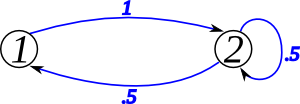
\includegraphics[width=.4\textwidth]{images/09mc2}
	\caption{Two state Markov chain.}
	\label{fig:09mc2}
\end{figure}

\begin{example}
Let
$$\mathbb{P} = \left[\begin{array}{c c c} 0 & 1 & 0 \\ \frac{1}{2} & 0 & \frac{1}{2} \\ 0 & 1 & 0 \end{array}\right]$$
This Markov chain is irreducible. See Figure \ref{fig:09mc3}. Also, $d(i)=2 ~\forall i$. We also have
\begin{align*}
\begin{split}
p_0 &= \left[\begin{array}{c} q_1 \\ q_2 \\ q_3 \end{array}\right]
\end{split}
\begin{split}
p_1 &= \mathbb{P}^Tp_0 = \left[\begin{array}{c} \frac{q_2}{2} \\ q_1+q_3 \\ \frac{q_2}{2} \end{array}\right]
\end{split} \\
\begin{split}
p_2 &= \mathbb{P}^Tp_1 = \left[\begin{array}{c} \frac{q_1+q_3}{2} \\ q_2 \\ \frac{q_1+q_3}{2} \end{array}\right]
\end{split}
\begin{split}
p_3 &= \mathbb{P}^Tp_2 = \left[\begin{array}{c} \frac{q_2}{2} \\ q_1+q_3 \\ \frac{q_2}{2} \end{array}\right]
\end{split}
\end{align*}
Since $p_3=p_1 \therefore p_{2n}=p_2$, $p_{2n-1}=p_1 ~\forall n\geq1$ and the dynamics oscillate. Also, it can be seen that
\begin{align*}
\begin{split}
\mathbb{P}^2 = \left[\begin{array}{c c c} \frac{1}{2} & 0 & \frac{1}{2} \\ 0 & 1 & 0 \\ \frac{1}{2} & 0 & \frac{1}{2} \end{array}\right]
\end{split}
\begin{split}
\mathbb{P}^3 = \left[\begin{array}{c c c} 0 & 1 & 0 \\ \frac{1}{2} & 0 & \frac{1}{2} \\ 0 & 1 & 0 \end{array}\right]
\end{split}
\end{align*}
So $\mathbb{P}$ is periodic (oscillates) too.
$\lozenge$
\end{example}

\begin{figure}[ht!]
	\centering
	\includegraphics[width=.4\textwidth]{images/09mc3}
	\caption{Three state Markov chain.}
	\label{fig:09mc3}
\end{figure}

\subsection{Infinite Size Gets Strange}
See Figure \ref{fig:09mcinf}. Suppose
\begin{align*}
\begin{split}
p_0 = \left[\begin{array}{c} 1 \\ 0 \\ 0 \\ 0 \\ \vdots \end{array}\right],
p_1 = \left[\begin{array}{c} \frac{1}{4} \\ \frac{3}{4} \\ 0 \\ 0 \\ \vdots \end{array}\right],
p_2 = \left[\begin{array}{c} \frac{1}{4} \\ \frac{3}{16} \\ \frac{9}{16} \\ 0 \\ \vdots \end{array}\right],
\ldots
\end{split}
\end{align*}
This leads to $\sum p_{t_i}=1$, but $p_{t_i}\rightarrow 0 ~\forall i$ as $i\to\infty$.

\begin{figure}[ht!]
	\centering
	\includegraphics[width=.4\textwidth]{images/09mcinf}
	\caption{Infinite state Markov chain.}
	\label{fig:09mcinf}
\end{figure}

\begin{definition}
$\Pi\in S^N = S^{\#\mathbb{X}}$ such that $\Pi=\mathbb{P}^T\Pi$ is called a \textit{stationary distribution} for the Markov chain $(\mathbb{X},\mathbb{P})$.
\end{definition}

\begin{example}
Suppose
$$\bar{p}=\lim_{t\to\infty}p_t = \lim_{t\to\infty}(\mathbb{P}^T)^tp_0$$
then
$$\mathbb{P}^T\bar{p}=\lim_{t\to\infty}\mathbb{P}^T(\mathbb{P}^T)^tp_t = \lim_{t\to\infty}(\mathbb{P}^T)^{t+1}p_0=\bar{p}$$
$\therefore \bar{p}$ is a stationary distribution.
$\lozenge$
\end{example}


\end{document}

%%%%%%%%%%%%%%%%%%%%%%%%%%%%%%%%%%%%%%%%%%%%%%%%%%%%%%%%%%%%%